%************************************************
\chapter{Particle Detection with Liquid Xenon}

\label{ch:LXeTPCs} 
%************************************************

\section{Liquid Xenon as a Detector Medium}
Liquid xenon detectors are powerful tools for rare event searches. In particular, the dual phase \ac{LXe} \ac{TPC} has been very successful in accessing \ac{WIMP} parameter space and currently holds the worlds most sensitive limits on \ac{WIMP}s. This section describes the properties of \ac{LXe} and the basic principles of \ac{TPC}s that have allowed this technology to play a large role in the hunt for dark matter.

\subsection{Properties of Liquid Xenon}
Liquid xenon has many properties relevant to particle detection, particle identification, and also many properties related to the ease of detector operation:

\begin{itemize}
  \item The density of \ac{LXe} is 2.9~g/cm$^{3}$ at 170~K, much denser than other possible \ac{TPC} target materials, such as liquid argon which has density 1.4~g/cm$^{3}$ at 87~K. The advantage in this two-fold: (1) the same volume contains more kg of Xe than Ar, so for two detectors of the same volume, one filled with Xe and the other with Ar, both running for one year, the Xe detector has more exposure; (2) xenon's high density effectively stops external radiation, producing an ultra-low-background volume in the center of the detector where rare-event searches can be performed (this region is called the ``fiducial volume'').
  
  \item Xenon gas is easily liquefied with liquid nitrogen (77~K) or commercially available pulse tube refrigerators.

  \item Xenon has no long-lived radioisotopes that cause troublesome backgrounds. The one exception is the 2$\nu\beta\beta$ decay of $^{136}$Xe (natural abundance 8.875\%) with measured half-life of $2.1 \times 10^{21}$ years. The long half-life and relatively low abundance together result in a very low count rate, and the isotope can be used to search for neutrino-less double beta decay ($0\nu\beta\beta$).
  
  \item Xenon, as a noble element, is easily purified with a heated getter to rid electronegative impurities (e.g. O$_{2}$) that interfere with the ionization signal. 
  
  \item The comparatively large mass of xenon allows it to be purified of other noble gasses via gas chromatography \cite{LUXKrRemoval2018} and cryogenic distillation \cite{Xe1TKrRemoval2017}. As other noble gasses cannot be removed via getter, this feature is extremely useful in removing the troublesome background of $^{85}$Kr decay. $^{85}$Kr decays via beta emission to stable $^{85}$Rb with a half-life of 10.8 years and Q$_{\beta}$ = 687~keV. The decay proceeds directly to the $^{85}$Rb ground state with a branching ratio of 99.6\%. Since no de-excitation of $^{85}$Rb follows, this beta decay cannot be rejected as background by coincidence with a gamma, and relies purely on the ability to discriminate between WIMP-like \ac{NR} and beta- or gamma- produced \ac{ER}. While ER/NR discrimination is one of the features of \ac{LXe} \ac{TPC}s (described in section \ref{sec:er_nr_discrimination}), leakage of \ac{ER} events in to the \ac{NR} signal region can occur and the best mitigation is to remove as much of the  $^{85}$Kr as possible. Single-phase \ac{LXe} detectors, with no ER/NR discrimination, benefit greatly from the ability to remove $^{85}$Kr.
  
  \item Particles interacting in \ac{LXe} excite atoms and create electron ion-pairs, producing detectable quanta: scintillation photons and ionization electrons, respectively (described in section \ref{sec:signal_generation}).
  
  \item Xenon produces scintillation light of wavelength $\lambda$~=~178~nm (described in section \ref{sec:signal_generation}). Xenon is transparent to this wavelength so it can propagate freely and be directly detected with current \ac{PMT} technology, and doesn't require the use of e.g wavelength shifter. 
  
  \item Ionization electrons produced in particle interactions can be drifted and extracted into a gaseous region via applied electric fields, where they undergo proportional scintillation. By this method, a single electron is amplified many-fold into detectable photons. This basic operating principle of dual-phase \ac{TPC}s makes even a single ionization electron detectable. 
  
  \item Xenon has high light and charge yields, and therefore a low threshold for producing detectable quanta. A useful quantity is the so-called `W-value' of \ac{LXe}: W = 13.7 $\pm$ 0.2 eV \cite{Dahl2009}. The W-value, analogous to a work-function, is a measure of the average energy expenditure to produce one quanta (scintillation photon or an ionization electron) from liquid xenon. 
  
  \item \ac{LXe} \ac{TPC}s are easily scalable: creating a large homogenous volume is straightforward. In contrast, solid state detectors, such as cryogenic Ge, are more difficult to scale up directly and require instead the production of multiple small modules (O(10)~cm) which each must be instrumented separately.  
    
\end{itemize}


\subsection{Scintillation and Ionization Signal Generation}
\label{sec:signal_generation}
A particle can interact with a xenon atom through interaction with an orbiting electron, creating an \ac{ER}, or though an interaction with the xenon nucleus, where the nucleus is imparted with momentum and recoils, \ac{NR}. Some energy is lost to atomic motion (heat). The recoiling electron or nucleus loses energy via interaction with neighboring xenon atoms, creating more excited atoms and electron-ion pairs. The excited xenon atoms, Xe$^{*}$, combine with other atoms to form an excited dimer, or excitons, Xe$_{2}^{*}$. The excited dimer forms two states: a triplet and a singlet, which de-excite with the emission of a 178~nm photon. The lifetimes of the triplet and singlet are measured to be 24~ns and 3~ns, respectively \cite{Mock2014}. Since the scintillation light is produced by the excimer, which has a different electronic structure than atomic xenon, the light is free to propagate through the detector and will not be absorbed by the atomic xenon. The Xe$^{+}$ ions of the electron-ion pairs combine with other Xe atoms to form dimers Xe$_{2}^{+}$, and these dimers can combine with electrons (from the electron-ion pairs) to form excitons, Xe$_{2}^{*}$, which then decay and produce additional 178~nm scintillation photons. This process is called recombination. If no electric field is applied, all electron-ion pairs recombine to produce additional scintillation photons. If an external electric field is present, some electrons can be drifted away from the interaction site to be detected with other methods. 

The sensitivity of liquid xenon detectors to low energy recoils depends on their ability to detect the 178~nm scintillation photons with high-efficiency. High \ac{QE} \ac{PMT}s constructed with ultra-low radioactivity materials are the go-to instrument for this purpose. In addition to high-efficiency photon-detectors, liquid xenon detectors must also have high geometrical light collection efficiency to optimize sensitivity. Single-phase liquid xenon detectors, where no electric field is applied, maximize light-collection by with a spherical geometry, endeavoring to cover 4$\pi$ steradians surrounding the \ac{LXe}. The XMASS detector uses spherical geometry to accomplish photocathode coverage of \~62\%, and two types of Hamamatsu \ac{PMT}s (R10789-11 and R10789-11MOD) with \ac{QE} of 28\%, and quote a signal collection efficiency of 20\% \cite{Abe2013}, \cite{XMASSCollaboration2018}. Dual-phase \ac{TPC} detectors are lined with \ac{PTFE} to take advantage of its extremely high (~99\%) reflectivity for 178~nm light in \ac{LXe} \cite{Neves2017}. The LUX detector uses a cylindrical geometry, with all non-light-collectiing surfaces lined with \ac{PTFE}, and Hamamatsu R8778 \ac{PMT}s (\ac{QE} of 33\%) only on the top and bottom of the detector (low photocathode coverage), to accomplish a light collection efficiency of 90\% \cite{Faham2014}.

If the detector is a \ac{TPC} the ionization electrons are drifted away from the interaction site to be detected. Single phase \ac{TPC} employ thin wires to collect the ionization electrons. For example, the EXO-200 experiment is a single-phase liquid xenon \ac{TPC} that uses crossed-wire planes to collect the ionization electrons and avalanche photodiodes to collect the scintillation photons \cite{Auger2012}. LUX is a dual-phase xenon \ac{TPC}, where ionization electrons produced in the large liquid region are drifted and extracted into gaseous xenon via applied electric fields, where they undergo proportional scintillation. The proportional scintillation light is the same 178~nm wavelength as scintillation in the liquid produced in the liquid, and it is similarly collected via high \ac{QE} \ac{PMT}s.

In addition to light-collection efficiency, the sensitivity of \ac{TPC} xenon detectors also depends on their ability to collect signal from the ionization electrons. There are challenges in delivering \ac{HV} to liquid xenon in order to set up the electric field which drifts the ionization electrons (some of these challenges are explained in Chapter \ref{ch:testbed}). Additionally, electronegative impurities such as oxygen (O$_{2}$) present in the detector attract and capture ionization electrons as they drift, eating away the ionization signal. These non-noble impurities are removed by constantly circulating the xenon through a heated zirconium getter and returning it to the detection volume. Purification through a getter must be done in gaseous phase, so liquid xenon removed from the detection volume is evaporated, passed through the getter via a circulation system, and re-condensed into the detection volume. 


\section{Dual-Phase Xenon Time Projection Chamber}
A particle interacting in a noble liquid or gas target deposits energy into scintillation and ionization channels (Section \ref{sec:signal_generation}). The basic operating principle of \ac{TPC}s is to drift the ionization electrons away from the interaction site and detect them at a later time than the scintillation signal is detected. A dual phase liquid xenon \ac{TPC} is a type of \ac{TPC} with a large liquid target volume and a small region of xenon vapor above the liquid volume, instrumented with light sensors (typically \ac{PMT}s). A particle interacting in the liquid target produces both scintillation photons and ionization electrons at the interaction site. The scintillation photons are promptly detected by the \ac{PMT}s, this primary signal is called S1. The ionization electrons are drifted upward to the gas region by an applied electric field, and extracted across the liquid-gas boundary by a higher electric field, where they undergo proportional scintillation and produce a second signal detected by the \ac{PMT}s, called S2. The field is supplied by a series of electrodes, composed of wire planes, grids, or chemically etched meshes, held at constant voltages. The bottom-most field-producing electrode is called the cathode, at the top of the liquid region is the gate or extraction electrode, followed O(1)~cm by the anode. The liquid region is often referred to as the `drift region' and region between the gate and anode is referred to as the `extraction region'. The drift region takes up by far more volume than the extraction region. The electrons are extracted from liquid to gas with some efficiency, called the \ac{EEE}. This efficiency plays an important role in the operation of dual-phase \ac{LXe} \ac{TPC}s, and is discussed further in  \textbf{E-Train CHAPTER}.

The S2 in a dual-phase \ac{TPC} plays two important roles: (i) internal amplification of the signal, whereby a few electrons are transformed into O(10) times as many photons (ii) $(x,y)$ localization via \ac{PMT} hit pattern. The time spacing of the S1 and S2 signals can be converted to depth ($z$) of the interaction, providing full $(x,y,z)$-reconstruction of the interaction position.

\begin{figure}[htbp]
\begin{center}
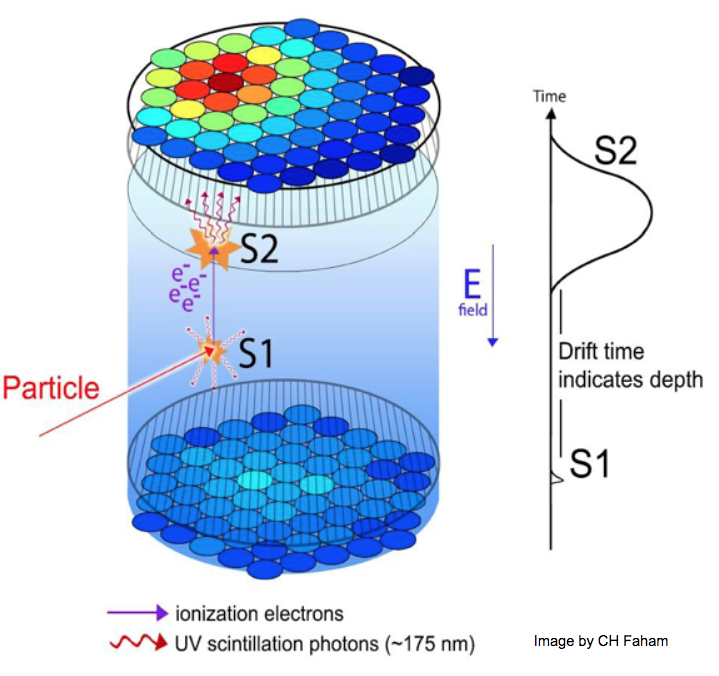
\includegraphics[width=\halffig]{figures/lxetpcs/TPC.png}
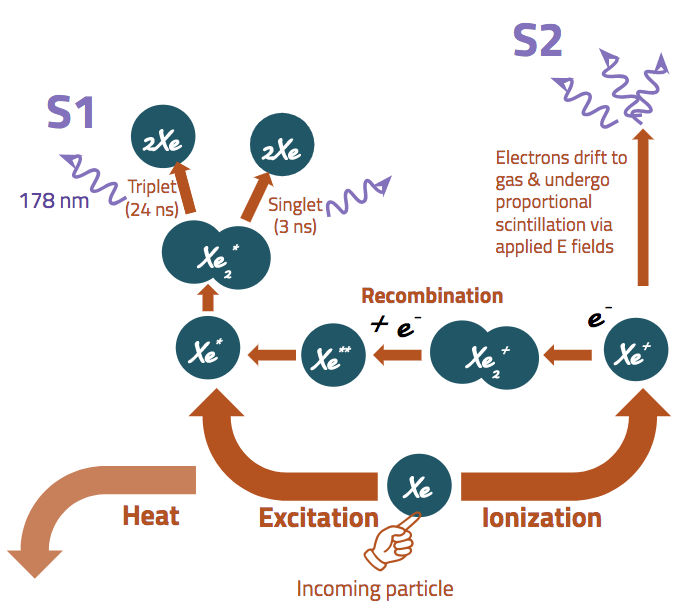
\includegraphics[width=\halffig]{figures/lxetpcs/signal_generation_in_lxe_tpcs.png}
\caption{ (left) Diagram of a dual-phase xenon time projection chamber. The time difference between S1 and S2 gives the depth ($z$) of the interaction, and $(x,y)$ is reconstructed from the S2 signal. (right) Diagram summarizing the generation of the scintillation and ionization signal generation in dual-phase xenon time projection chambers.}
\label{fig:tpc}
\end{center}
\end{figure}


The \ac{LUX} detector is a dual-phase liquid xenon TPC.

\subsection{Energy Reconstruction}
Energy reconstruction in dual-phase xenon \ac{TPC}s comes from the measurable quantities, S1 and S2, but begins with the number of excitons $n_{ex}$  and electron-ions pairs $n_{i}$ generated at the interaction site. 
\begin{equation}
E = f W (n_{ex} + n_{i} )
\end{equation}

where $E$ is the deposited energy. $W$ is the average energy needed to produce a single excited or ionized atom, $W = 13.7 \pm 0.2$~eV \cite{Mock2014}. The quenching factor, $f$ is 1 for electronic recoils but $f \neq 1$ for nuclear recoils. For now, take the case of electronic recoils and set $f=1$. This equation can be rewritten:

\begin{equation}
E = W (1 + \frac{n_{ex}}{n_{i}} ) n_{i}
\end{equation}

The ratio of excitons to ions is constant for electron recoils $n_{ex}/{n_{i}} = 0.2$ \cite{LUX:YieldsAndRecombination}. As discussed in Section \label{sec:signal_generation}, each exciton deexcites, emitting a 178~nm photon, some fraction $r$ of the initial electron-ion pairs recombine and form additional excitons. The total number of prompt scintillation photons created by the interaction is then:

\begin{equation}
n_{\gamma} = (r + \frac{n_{ex}}{n_{i}} ) n_{i}
\end{equation}

And the total number of electrons created by interaction site (electrons escaping recombination) is:

\begin{equation}
n_{e} = (1 - r ) n_{i}
\end{equation}

Thus, the effect of recombination is to ``trade-out'' electrons for photons, but the total number of quanta is conserved. These two quantities, $n_{\gamma}$  and $n_{e}$ relate directly to the observable S1 and S2 signals:

 \begin{equation}
E = W (n_{\gamma} + n_{e} )
   = W (\frac{S1}{g_{1}} + \frac{S2}{g_{2}})
\end{equation}

where S2 and S2 are in units of detected photons, and $g_{1}$ and $g_{2}$ are detector gains in units of detected photons (phd) / quanta. $g_{1}$ is the detection efficiency for the prompt scintillation photons: it is a product of the the average a geometrical light collection efficiency and the average \ac{PMT} \ac{QE}. Typical values for $g_{1}$ are in the range of 0.01-0.02. $g_{2}$ is the analogous quantity for S2 proportional scintillation light: it is a product of the \ac{EEE} and the average number of detected photons produced by one extracted electron. Typical values for $g_{2}$ are in the range 10-60.


\section{Dual-Phase Xenon TPCs for Dark Matter Detection}

\subsection{Optimization for WIMPs}

\subsubsection{ER, NR Discrimination}
\label{sec:er_nr_discrimination}

\subsubsection{WIMP Rates and Cross section}

\subsection{LIP Search Ability}


%*****************************************
%*****************************************
%*****************************************
%*****************************************
%*****************************************

